% TFG - José Ángel Martín Baos. Escuela Superior de Informática. 2018
%%%% CHAPTER: Methodology %%%
% !TeX spellcheck = en_GB

\chapter{Methodology}
\label{chap:methodology}

\drop{I}{n} order to carry out this project, a working methodology should be chosen and followed throughout the development of this \ac{BSc.} thesis. In particular, \emword{Scrum} is used as project management methodology and \emword{Kanban} is adopted to manage the progress of the project. In addition, the iterative and incremental software development methodology is used, where the product is developed in several increments and each increment is executed in iterative cycles. To end with, the details of the different means and resources used are also described.


\section{Agile methodologies}

In the last few years, the number of companies, with different size and from different areas, using agile development methodologies has increased considerably. These methodologies are not only used by the software development companies, but also they are used by a wide range of companies. In the software engineering field, agile methodologies gain a lot of importance due to the complexity sometimes needed to specify the different requirements of a product in an unique phase. Agile methodologies makes a great difference with respect to \emword{Waterfall} model where carrying out a change once the product is almost finished is very costly.

In an agile project it is sought to divide the tasks of the software project in increments with a minimum planning and a short duration (normally between one and four weeks). Each iteration produces an operational prototype that is revised together with the client. Therefore, we can affirm that the life cycle of the agile methodologies is iterative and incremental.

Some examples of agile methodologies could be:
\begin{multicols}{2}
	\begin{itemize}
		\item \emword{Scrum} \cite{ScrumGuide}
		\item Adaptive Software Development \\ \cite{ASD}
		\item Extreme Programming (XP) \cite{XPProgramming}
		\item Open Unified Process (OpenUP) \\ \cite{Bal07}
		\item Feature-Driven Development \cite{FDD}
		\item Lean \cite{PP03}
	\end{itemize}
\end{multicols}

In April 2017 the \emph{11th annual state or agile survey} \cite{AnualStateAgile} produced a listing with the most applied agile methodologies as shown in Figure \ref{fig:5-AgileMethodologyUsed}. The most used agile methodology is \emword{Scrum} with a 58\% of the total number of organizations using such methodology.

In our view, \emword{Scrum} fits nicely with the problem dealt in this \ac{BSc.} thesis as this project consist on a hardware-software system organised in several stages. Furthermore, as consequence of being one of the most used agile methodologies, lot of literature has been written about it, for this reason, \emword{Scrum} has been chosen. Specifically, \emword{Scrum} methodology \cite{ScrumGuide} has been adapted to an one-person development. To manage the progress of the project graphically the Kanban technique with the tool Trello\footnote{Trello website: \url{www.trello.com} \label{footnote-1}} is used.

\begin{figure}[!h]
	\begin{center}
		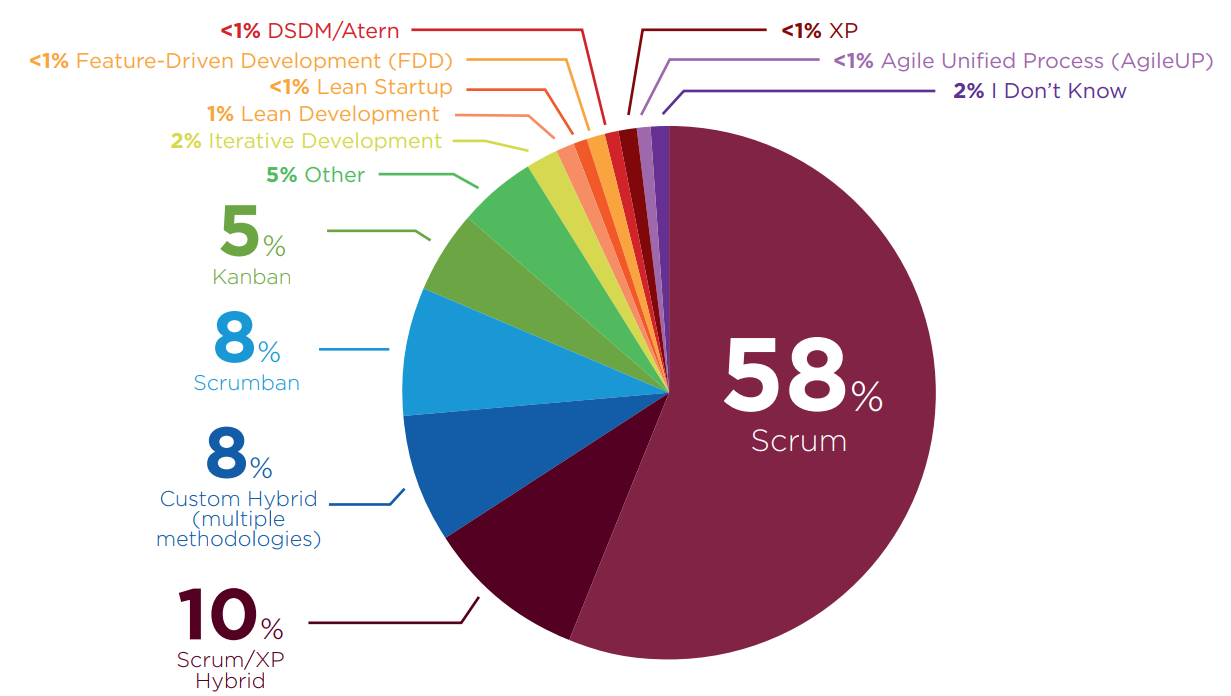
\includegraphics[width=1\textwidth]{5-AgileMethodologyUsed.png}
		\caption{Most used agile methodologies}{Source: The \emph{11th annual state or agile survey}}
		\label{fig:5-AgileMethodologyUsed}
	\end{center}
\end{figure}

Now, a general description of \emword{Scrum} is exposed.


\subsection{Scrum}

\emword{Scrum} \cite{ScrumGuide} is an agile project management methodology not necessarily related with software projects. \emword{Scrum} has two main characteristics: The first one is that the development of the software is carried out in incremental iterations, whilst the second one is that coordination meetings are held throughout the project.
In \emword{Scrum}, the product is developed in series with a duration from one to four weeks called \emword{Sprints}. The different requirements are captured as elements of a list called \emword{product backlog} which is created at the beginning of the project. Figure \ref{fig:5-ScrumSprints} represents the complete \emword{Scrum} life cycle.

\begin{figure}[!h]
	\begin{center}
		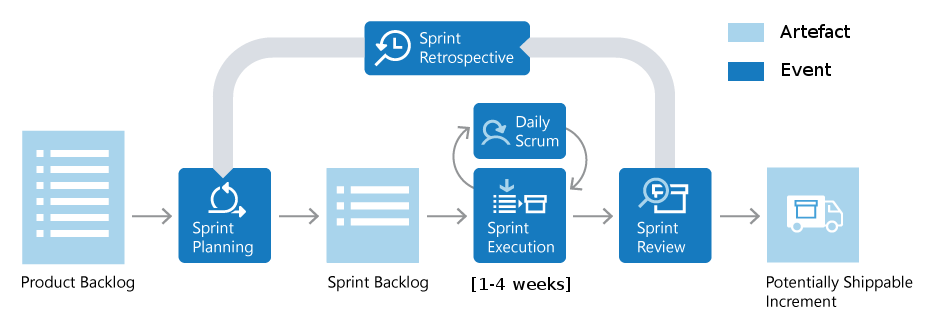
\includegraphics[width=1\textwidth]{5-ScrumSprints-v2.png}	
		\caption{Scrum life cycle}{Source: \url{https://www.visualstudio.com/es/learn/what-is-scrum}}
		\label{fig:5-ScrumSprints}
	\end{center}
\end{figure}


\subsubsection{Scrum Team} \label{5-ScrumTeam}
\emword{Scrum} Teams are self-organizing, cross-functional, non-distributed and must have an optimal size. The team model in \emword{Scrum} is designed to optimize flexibility, creativity, and productivity and its different roles are:

\begin{itemize}
	\item \emlst{Product owner.} Is responsible for maximizing the value of the product and the work of the	development team. This person is also responsible of establishing the user stories, assigning them a priority and classifying them in the product backlog. The product owner must have a very clear perspective of the product which will be developed and must transmit it to the development team.
	
	\item \emlst{Scrum master.} Is responsible for ensuring that the \emword{Scrum} is understood by all the members and that the \emword{Scrum} team adheres to \emword{Scrum} theory, practices, and rules. 
	
	\item \emlst{Development team.} Consists of professionals who do the work of delivering a potentially releasable increment of “Done” product at the end of each Sprint. It is recommended that they work full time, in the same place and they should not change during a Sprint.
\end{itemize}


\subsubsection{The Sprint}

In agile methodologies, the requirements that must fit the software which will be developed are collected into user stories. The user stories \cite{Coh04} are a brief description of the software functionality as the user perceives them. A Sprint is a time block with a duration from one to four weeks in which a product increment is obtained. Therefore, each Sprint can be considered as a project itself. A new Sprint starts immediately after the conclusion of the previous Sprint. The \emph{Sprint goal} is the objective set for the Sprint that can be met through the implementation of product backlog. No changes can be made in the Sprint goal during the Sprint execution. 


\subsubsection{Scrum events}
Some events are planned with a fixed duration and a concrete objective in order to minimize the need for meetings not defined previously. These events are the following ones:

\begin{itemize}
	\item \emlst{Sprint planning meeting.} Consists of a meeting carried out at the start of each Sprint where the elements from the product backlog to be developed are selected. Therefore, the Sprint backlog is created. This meeting should not last more than one day.
	
	\item \emlst{Daily Scrum.} Consist of daily meetings with a duration of less than fifteen minutes where the development team can synchronize their activities and create a plan for the next 24 hours. This is done by inspecting the work since the last daily Scrum and forecasting the work that could be done before the next one.
	
	\item \emlst{Sprint review.} Consist of a informal meeting held at the end of the Sprint to inspect the increment and adapt the product backlog if needed. During the Sprint review, the Scrum team and the stakeholders collaborate about what was done in the Sprint.
	
	\item \emlst{Sprint retrospective.} It is an opportunity for the Scrum team to inspect itself and create a plan for improvements to be enacted during the next Sprint. It has a maximum duration of three hours and takes place between the Sprint review meeting and the next Sprint planning meeting.
\end{itemize}


\subsubsection{Scrum artefacts}
When using \emword{Scrum}, some outputs are obtained known as \emword{Artefacts}. They represent work or value to provide transparency and opportunities for inspection and adaptation. Figure \ref{fig:5-ScrumSprints} shows the different artefacts and the moment in the Scrum life cycle when they are obtained.

\begin{itemize}
	\item \emlst{Product backlog.} Consist of an ordered list of requirements or user stories that will be included in the software product in the increments. This list is created by the Product owner. This list is never complete, therefore, it can change during the project to identify what the product needs. 
	
	\item \emlst{Sprint backlog.} It is a subset of the elements contained in the product backlog. It consists of an ordered list of user stories to be developed during this Sprint.
	
	\item \emlst{Product increment.} The increment is the sum of all the product backlog items that has been completed during a Sprint and the value of the increments of all the previous Sprints.
\end{itemize}

Heretofore, \emword{Scrum} project management methodology has been explained, besides the team needed for using it, the events organized and the artefacts produced. In the next section Kanban technique will be explained.


\section{Kanban}

Kanban \cite{Gar11,KS10} is a Japanese technique for managing the progress of the project. It was invented by Toyota and was used to control the progress of their work in the production line. Therefore, Kanban is not a specific software development technique, nevertheless, in the last few years it has been used in the management of software projects.

Kanban allows the development team to visualize the workflow of the different tasks. Normally, consists in using a slate board with three columns: \emph{To Do}, \emph{Doing} and \emph{Done}, that represents the different phases a task passes until it is completed. Each task in which a Sprint is divided is considered as a card which is put into the slate board. An example of this concept can be seen in Figure \ref{fig:5-KanbanBoard}.

To manage the Kanban Board, Trello is used, as it was previously indicated. This tool allows the creation of several boards. In each board many columns can be created with various tasks that can be moved from one column to another by means of a very friendly interface.

\begin{figure}[!h]
	\begin{center}
		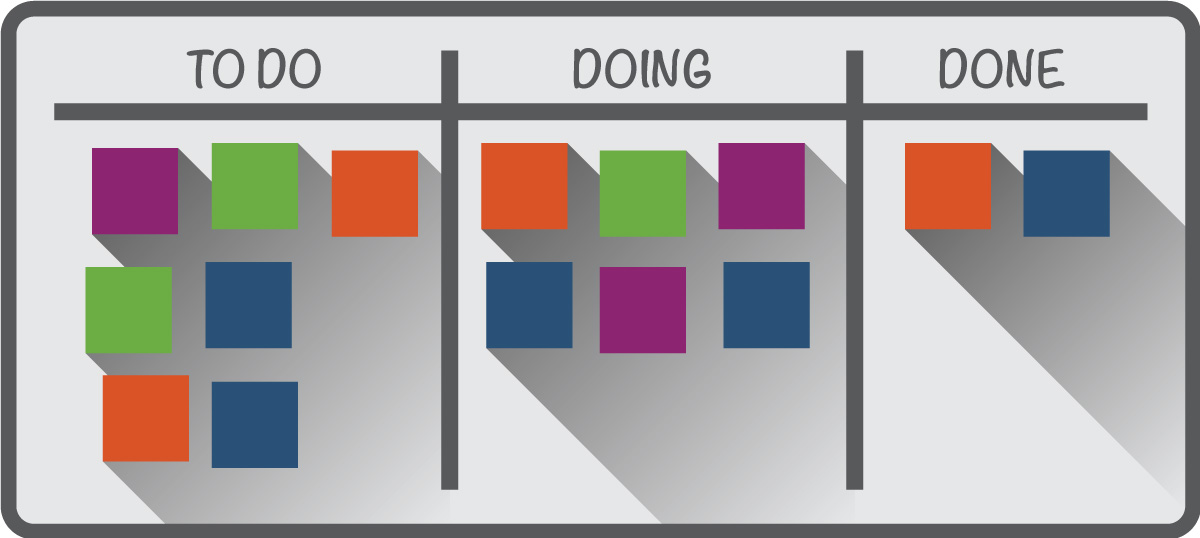
\includegraphics[width=0.8\textwidth]{5-KanbanBoard.jpg}
		\caption{Kanban Board}
		\label{fig:5-KanbanBoard}{Source: \url{www.qe2ingenieria.com}}
	\end{center}
\end{figure}

Up to this time, the project management methodology has been presented. Now, the development methodology will be introduced.


\section{Development methodology}
The development methodology is used by developers and engineers to write code, helping them in the process and giving some guidelines when developing computer systems in order to maintain a high code quality. In this \ac{BSc.} thesis the iterative and incremental software development methodology is used. In this method of software development the project is divided into several blocks, which match with the temporal blocks defined in \emword{Scrum} \cite{ItIncr}. 

Each iteration of the iterative and incremental methodology can be considered as a project itself where a value must be added to the final product. For each of those iterations all the tasks necessary to complete it must be executed, incorporating analysis, design, coding and testing phases (this is the reason of being called iterative). Moreover, in each iteration the team must take the work done in the previous iterations and include new objectives and requirements or improve the ones that are already accomplished (this is the reason of being called incremental). Figure \ref{fig:5-Iterative-and-incremental} represents the iterative and incremental methodology flow.

\begin{figure}[!h]
	\begin{center}
		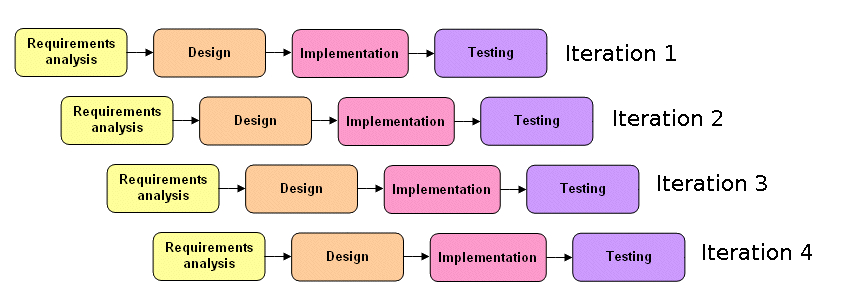
\includegraphics[width=0.9\textwidth]{5-Iterative-and-incremental.jpg}
		\caption{Iterative and incremental methodology flow}
		\label{fig:5-Iterative-and-incremental}{Adapted from  \url{http://www.technologyuk.net}}
	\end{center}
\end{figure}

Some of the advantages of using the iterative and incremental methodology are:
\begin{itemize}
	\item The end product is more adjusted to the client needs due to the fact that in each iteration a part of the product is obtained and it can be checked by the client and, therefore, some adjustments can be made in the following iterations.
	
	\item The changes that may appear during the project can be managed easier.
	
	\item Functional results are obtained since the firsts iterations.
	
	\item The client tend to involve itself more in the project. 
\end{itemize}

However, some disadvantages should be commented:
\begin{itemize}
	\item The result of each iteration must be an useful product, so that the result is really useful for the client.
	
	\item Each of the steps in an iteration are fixed and iterations cannot be overlapped.
	
	\item Some techniques must be used in order to accomplish changes in the product easily, without incrementing the complexity of the project.
\end{itemize}


\section{Resources}
In this section we are going to describe the different technologies that are employed during the development of this \ac{BSc.} thesis.

\subsection{Hardware resources}
Now, the different hardware resources employed in the \ac{BSc.} thesis are detailed. These include the computer used to develop the \ac{BSc.} Thesis, the Raspberry Pi and the different peripherals attached to it. Figure \ref{fig:5-Foto_zulo} shows the different hardware resources before starting the project.


\begin{figure}[!h]
	\begin{center}
		\includegraphics[width=0.96\textwidth]{5-Foto_zulo.JPG}
		\caption{Hardware resources}
		\label{fig:5-Foto_zulo}
	\end{center}
\end{figure}


\begin{itemize}
	\item \emlst{Development computer.} The personal computer of the student has been employed for this purpose. The spec table is shown in Table \ref{tab:development-computer-spec-table}.
	
	\begin{table}[!h]
		\centering
		{\small
			\begin{tabular}{ |l|l|}
	\hline
	\rowcolor{tabheadbg}
	\multicolumn{2}{|c|}{\textscale{.8}{\textbf{Development computer (\emph{draco}) specs}}} \\
	\hline
	Model						& Asus Zeenbook UX430UA \\
	\hline
	Processor					& Intel® Core™ i7-7500U CPU at 2.70GHz $\times$ 4 \\
	\hline
	RAM memory 					& 8 GB \\
	\hline 
	Hard drive					& 512 GB HDD \\
	\hline
	First Operating System		& Ubuntu 16.04.3 LTS \\
	\hline
	Second Operating System		& Windows 10 \\
	\hline

\end{tabular}
		}
		\caption{Development computer spec table}
		\label{tab:development-computer-spec-table}
	\end{table}
	
	\item \emlst{Raspberry Pi 3.} The Raspberry Pi is a low cost, credit-card sized computer. The Raspberry Pi 3 is the third-generation Raspberry Pi. Table \ref{tab:raspberry-pi3-spec-table} shows its spec table. With this computer a memory card is also needed. The one used is the \emph{Samsung SDHC EVO 8gb Class 10+}.
	
	\begin{table}[!h]
		\centering
		{\small
			%\begin{tabular}{ |l|l|l|}
%	\hline
%	\rowcolor{tabheadbg}
%	\multicolumn{3}{|c|}{\textscale{.8}{\textbf{Raspberry Pi 3 Model B specs}}} \\
%	\hline
%	Price						& $\sim$35\euro{} \\
%	\hline
%	SoC							& Broadcom BCM2837 \\
%	\hline
%	Processor					& Quad Core ARM Cortex A53 (ARMv8) at 1.2GHz 64bit \\
%	\hline
%	RAM memory 					& 1 GB \\
%	\hline 
%	GPIO pins					& 40 \\
%	\hline
%	\multirow{7}{*}{External ports}
%		& HDMI \\ 
%		& CSI camera port \\ 
%		& DSI display port \\ 
%		& Micro SD port \\
%		& 4 $\times$ USB 2 ports \\
%		& Ethernet port \\
%		& Audio jack 3,5 mm \\
%	\hline
%	\multirow{2}{*}{Wireless connections}
%	& BCM43438 wireless LAN  \\ 
%	& Bluetooth Low Energy (BLE) \\
%	\hline
%
%\end{tabular}

\begin{tabular}{ |l|l|l|}
	\hline
	\rowcolor{tabheadbg}
	\multicolumn{3}{|c|}{\textscale{.8}{\textbf{Raspberry Pi 3 Model B specs}}} \\
			\hline
	Price                                 & $\sim$35\euro{}                                  & \multirow{14}{*}{
		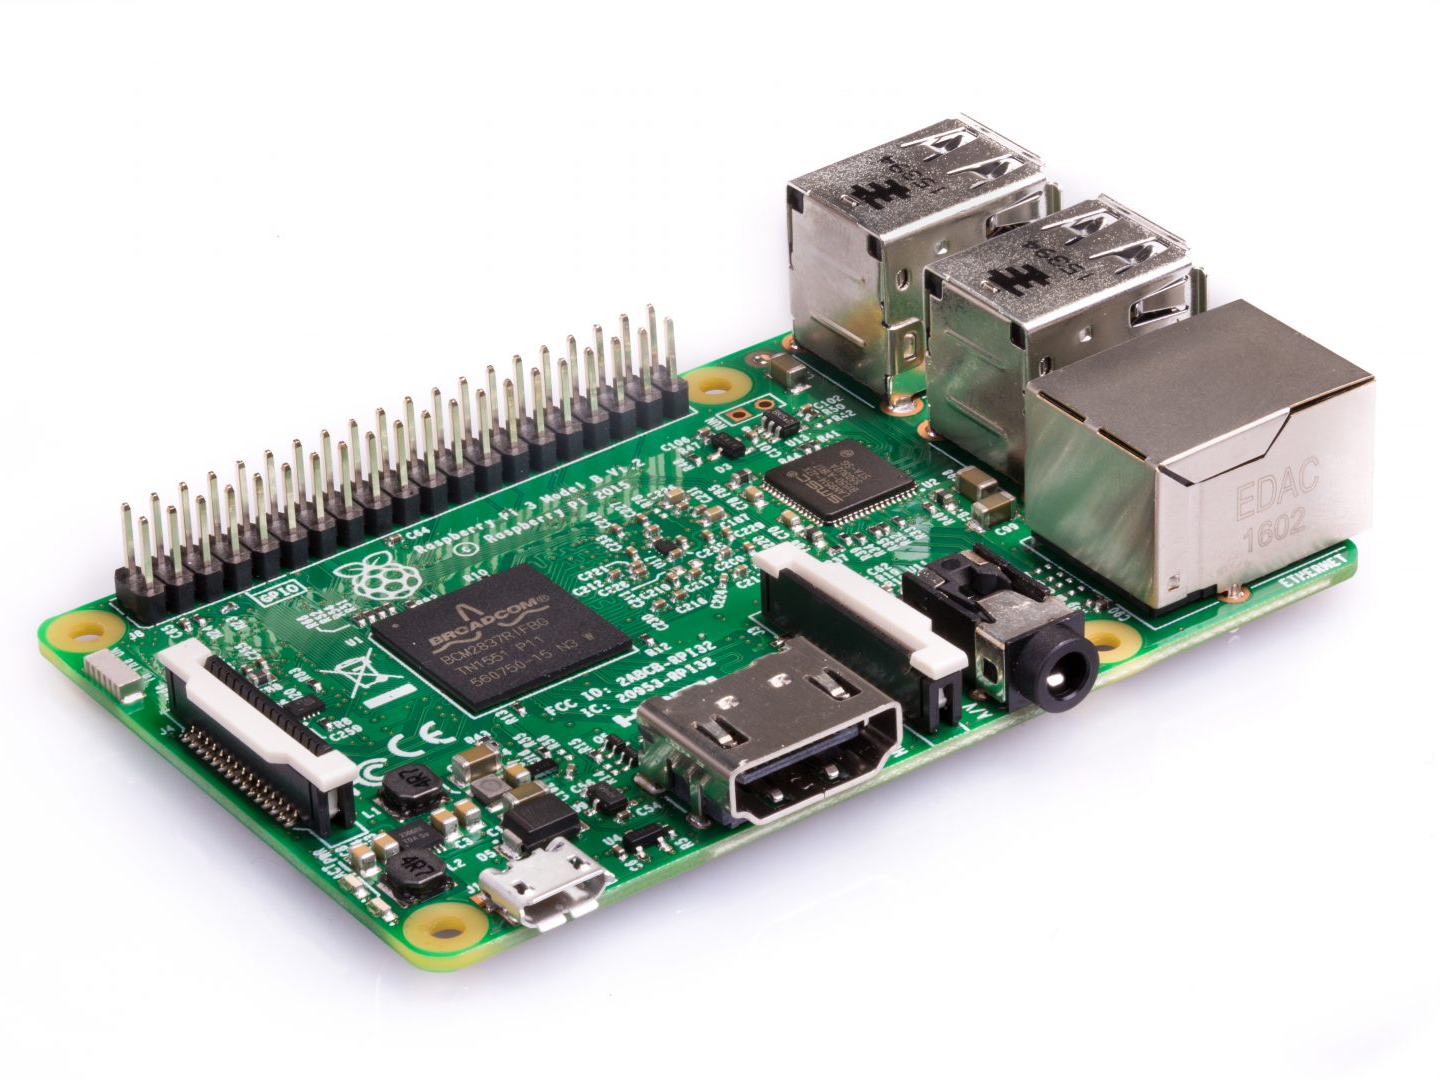
\includegraphics[width=0.36\textwidth]{5-RaspberryPi3.jpg}
	} \\ \cline{1-2}
	SoC                                   & Broadcom BCM2837                                 &                         \\ \cline{1-2}
	Processor                             & Quad Core ARM Cortex A53 				 &                         \\ 
			                              & (ARMv8) at 1.2GHz 64bit 								 &                         \\ \cline{1-2}
	RAM memory                            & 1 GB                                             &                         \\ \cline{1-2}
	GPIO pins                             & 40                                               &                         \\ \cline{1-2}
	\multirow{7}{*}{External ports}       & HDMI                                             &                         \\
	& CSI camera port                                  &                         \\
	& DSI display port                                 &                         \\
	& Micro SD port                                    &                         \\
	& 4 × USB 2 ports                                  &                         \\
	& Ethernet port                                    &                         \\
	& Audio jack 3,5 mm                                &                         \\ \cline{1-2}
	\multirow{2}{*}{Wireless connections} & BCM43438 wireless LAN                            &                         \\ \cline{2-2}
	& Bluetooth Low Energy (BLE)                       &                         \\ \hline
	
	
\end{tabular}

		}
		\caption{Raspberry pi 3 spec table}
		\label{tab:raspberry-pi3-spec-table}
	\end{table}
	
	\item \emlst{Raspberry Pi Camera Module V2 \cite{PiCameraDoc}.} It is a hardware module that allows the Raspberry Pi to capture pictures and record videos using the CSI port. The camera used is the \emph{PI NOIR CAMERA V2}.\footnote{More information in https://www.raspberrypi.org/products/pi-noir-camera-v2/} The table \ref{tab:raspberry-pi3-camera-specs} shows its specs. \label{itm:Pi-camera-module-v2}
	
	\begin{table}[!h]
		\centering
		{\small
			%\begin{tabular}{ |l|l|}
%	\hline
%	\rowcolor{tabheadbg}
%	\multicolumn{2}{|c|}{\textscale{.8}{\textbf{Pi NoIR Camera V2 specs}}} \\
%	\hline
%	Price						& $\sim$25\euro{} \\
%	\hline
%	Weight						& 3g \\
%	\hline
%	Resolution					& 8 Megapixels \\
%	\hline 
%	Dimensions					& 25$\times$24$\times$9 mm \\
%	\hline	
%	Sensor						& Sony IMX219 \\
%	\hline
%	\multirow{3}{*}{Video modes}
%		& 1080$\times$120p at 30 fps \\ 
%		& 720$\times$480p at 60 fps\\ 
%		& 640$\times$480p at 60$/$90 fps \\ 
%	\hline
%	Additional information		& No Infrared filter (NoIR) \\
%	\hline
%\end{tabular}

% Please add the following required packages to your document preamble:
% \usepackage{multirow}


\begin{tabular}{|l|l|l|}
	\hline
	\rowcolor{tabheadbg}
	\multicolumn{3}{|l|}{\textscale{.8}{\textbf{Pi NoIR Camera V2 specs}}}                       \\ \hline
	Price                        & $\sim$25\euro{}                     & \multirow{9}{*}{
		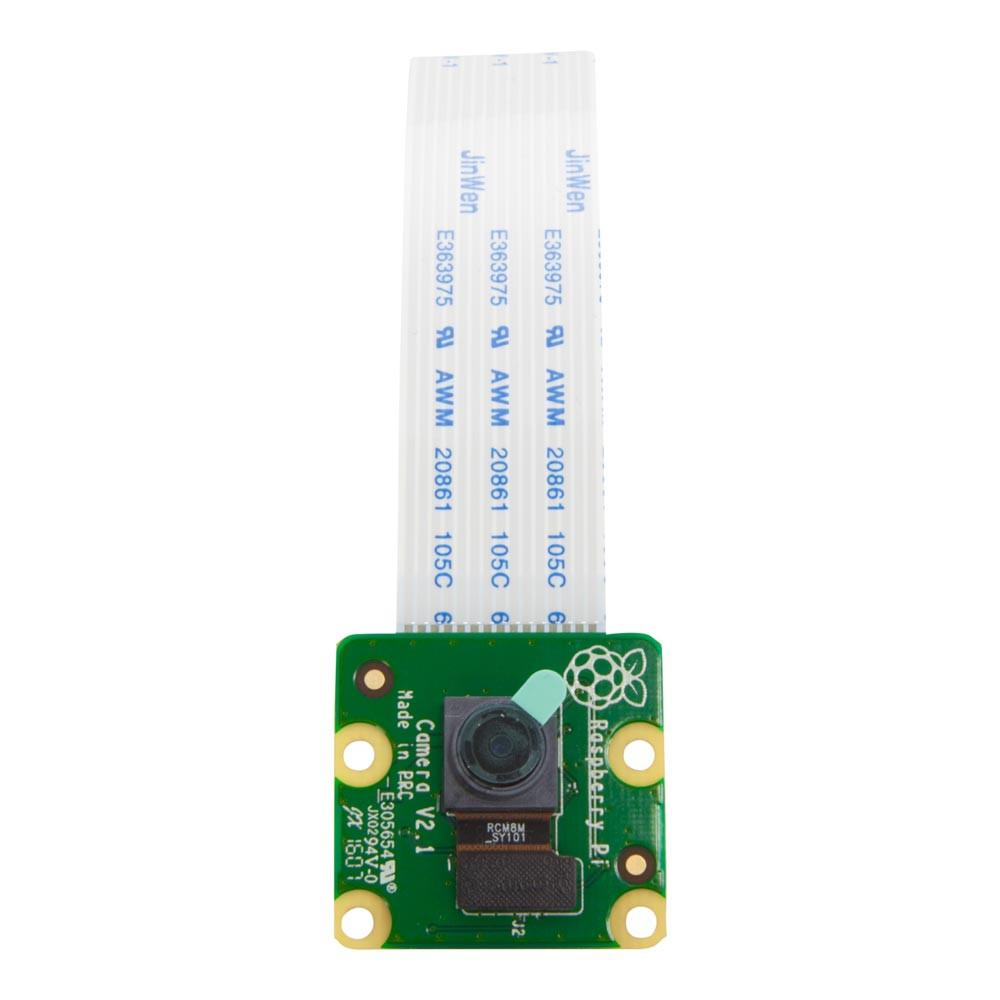
\includegraphics[width=0.28\textwidth]{5-PiCamera.jpg}
	} \\ \cline{1-2}
	Weight                       & 3g                        &                   \\ \cline{1-2}
	Resolution                   & 8 Megapixels              &                   \\ \cline{1-2}
	Dimensions                   & 25×24×9 mm                &                   \\ \cline{1-2}
	Sensor                       & Sony IMX219               &                   \\ \cline{1-2}
	\multirow{3}{*}{Video modes} & 1080p at 30 fps           &                   \\
	& 720p at 60 fps            &                   \\
	& 640x480p at 60/90 fps     &                   \\ \cline{1-2}
	Additional information       & No Infrared filter (NoIR) &                   \\ \hline
\end{tabular}
		}
		\caption{Pi NoIR Camera V2 spec table}
		\label{tab:raspberry-pi3-camera-specs}
	\end{table}

	\item \emlst{Sense HAT \cite{SenseHAT}.} It is an add-on board which is placed on top of the Raspberry Pi board. It was made for the Astro Pi mission which took place in December 2015. This board is composed by several components: 8x8 RGB LED matrix, five-button joystick and some sensors (temperature, humidity, barometric pressure, magnetometer, accelerometer and gyroscope).
	
	\item \emlst{Power bank battery.} The Raspberry Pi board is going to be powered using a power bank battery. The one used has a capacity of 10000 mAh and provide a maximum amperage of 2.1 amps at 5 volts.
	
	\item \emlst{MQ-7 Sensor. \cite{MQ7}} This sensor is able to measure Carbon Monoxide (CO) concentrations in the air. The MQ-7 can detect concentrations anywhere from 20 to 2000 ppm (parts per million) and has a fast response time. This sensor works with an input voltage of 5 volts and provide an analog output, therefore an anaglog to digital converter is needed.
	
	\item \emlst{MQ-2 Sensor \cite{MQ2}.} This sensor is able to measure methane, butane, petroleum gas and smoke in concentrations between 300 to 10000 ppm. As the previous sensor, this one also works with a voltage of 5 volts and provide an analog output.
	
	\item \emlst{Analog-to-digital-converter \cite{ADC}.} Ananalog-to-digital converter (ADC) is a system that converts an analog signal into a digital signal. Therefore, the input analog current is converted to a digital number proportional to the magnitude of the current that can be understood by a digital system.	
	
	\item \emlst{LM317 \cite{LM317}.} An electronic device which is capable of supplying more than 1.5 Ampers over an output voltage range of 1.25 to 37 Volts.
	
\end{itemize} 



\subsection{Software resources}
In this part the different software resources employed are described. These include the \ac{OS}, programming languages, libraries, the different development tools and the software used to generate the documentation as shown in Figure \ref{fig:5-SoftwareResources}.

\begin{figure}[!h]
	\begin{center}
		\includegraphics[width=0.92\textwidth]{5-SoftwareResources.pdf}
		\caption{Software resources}
		\label{fig:5-SoftwareResources}
	\end{center}
\end{figure}


\textbf{Operating Systems:}
\begin{itemize}
	\item \emlst{Ubuntu 16.04.3 LTS.} Ubuntu is a popular \ac{OS} based on \ac{GNU}$/$Linux. Ubuntu is one of the most used Linux distributions and it is normally used for personal computers, but also for servers and \ac{IoT}. This \ac{OS} is used for developing the software in the student computer.
	
	\item \emlst{Debian 9 “Stretch”.} Debian is also a \ac{OS} based on \ac{GNU}$/$Linux. Debian has a big community form by developers and users, which maintain the software. It is used also for developing the software.
	
	\item \emlst{Raspbian.} Raspbian is a Debian-based \ac{OS} designed for running in the Raspberry Pi.
	
	
\end{itemize}

\textbf{Programming Languages:}
\begin{itemize}
	\item \emlst{Python 3 \cite{Dow12}.} Python is a high-level programming language. Python focuses on offering a simple syntax, as well as being an interpreted language, allowing it to be ideal for scripting and for developing applications in various areas and for most platforms. In addition, it is an \ac{OO} language and has efficient and high-level data structures. Python has been used because it has lot of support for Raspberry Pi. Moreover, the main libraries for the camera module of the Raspberry Pi are written in Python and can use the power of the NumPy scientific computation library.
	
	\item \emlst{HTML \cite{Duc11}.} Hypertext Markup Language or HTML is the most common markup language for the creation of webpages or web applications. Web browsers receive the HTML code from the web severs and render it into web pages that are displayed to the user.
	
	\item \emlst{CSS \cite{Duc11}.} Cascading Style Sheets or CSS is a style sheet language which is used to create rules that specify how the content of an element should appear in a web page.
	
	\item \emlst{JavaScript.} JavaScript or JS is a high-level interpreted programming language. I is commonly used in interactive webpages and it is a essential part of web applications. JS supports functional, imperative, object-oriented and event-driven programming styles. Initially, it was created to run on the client-side, but nowadays it is used also in the web servers.
	
\end{itemize}


\textbf{Database:}
\begin{itemize}
	\item \emlst{MySQL \cite{Bea05}.} MySQL is an open-source relational database management system. It use \ac{SQL} language internally to access and mange the database.
	
	\item \emlst{MySQL Workbench.} It is an unified visual tool which provides data modelling, SQL development and comprehensive administrations tools for MySQL database servers configuration and maintenance.  
	
\end{itemize}

\newpage
\textbf{Libraries:}
\begin{itemize}
	\item \emlst{Python PiCamera \cite{PiCameraDoc}.} Python library for Python 2.7 or Python 3.2 (or above) which provides an interface for controlling the Raspberry Pi camera (PiCamera described in \ref{itm:Pi-camera-module-v2}).
	
	\item \emlst{Python NumPy \cite{NumPy}.} NumPy is a open-source scientific computing package for Python. It provides an easy and efficient way of working with multidimensional structures, such as the matrices of motion vectors used by H.264/AVC video format that is employed by the PiCamera library.
	
	\item \emlst{Python Matplotlib \cite{Hun07}.} Matplotlib is a Python 2D plotting library which produces quality figures in a variety of formats. For simple plotting the \emph{pyplot} module provides a MATLAB-like interface.
	
\end{itemize}

\textbf{Development tools:}
\begin{itemize}
	\item \emlst{Atom.} Atom is a free open-source text and source coder editor for macOS, Linux and Windows developed by GitHub. It allows to install a lot of plug-ins written in Node.js and has and embedded Git Control tool.\footnote{Available at \url{https://atom.io/}}
	
	\item \emlst{Vi.} Vi is a console text editor originally created for the Unix \ac{OS}. 
	
	\item \emlst{Git \cite{CS14}.} Git is a version control system for tracking changes in computer files and coordinating work on those files among multiple people. It is primarily used for source code management in software development, but it can be used to keep track of changes in any set of files.
	
	\item \emlst{GitHub.} GitHub is a web-based Git version control repository. It provides access control and several collaboration features such as bug tracking, feature requests, task management, and wikis for every project.\footnote{GitHub webpage: \url{https://github.com/}}	
	
\end{itemize}

\textbf{Software used for the documentation:}
\begin{itemize}
	\item \emlst{Trello.} Trello is a web tool which provides support for the Kanban technique allowing to manage the progress of the project. Trello provides the functionality to create boards composed by several lists with cards in them. For this project, a board has been created with 3 lists: \emph{To Do}, \emph{Doing} and \emph{Done}.$^{\ref{footnote-1}}$ Figure \ref{fig:5-Trello} shows a screen capture of Trello during the execution of User Story 3 in the Sprint 1.
	
	\begin{figure}[!h]
		\begin{center}
			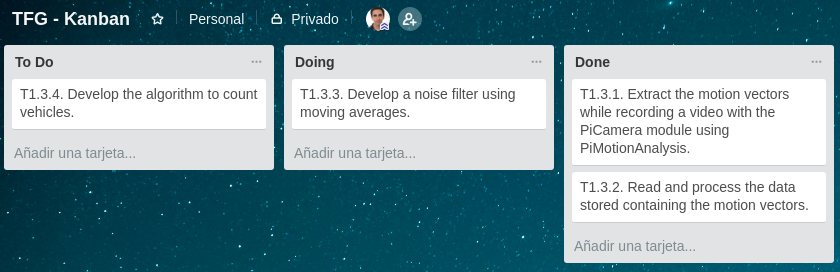
\includegraphics[width=0.96\textwidth]{5-Trello.png}
			\caption{Kanban board on Trello during the execution of User Story 3}
			\label{fig:5-Trello}
		\end{center}
	\end{figure}
	
	\item \emlst{\LaTeX{} \cite{Kot11}.} \LaTeX{} is a software for typesetting documents. It is not a word processor, but is used as a document markup language. \LaTeX{} is free, open source and provide great typographic quality on the documents, which makes it ideal for composing scientific documents. It is based on the \TeX{} typesetting engine created by Donald Knuth.
	
	\item \emlst{TeXstudio.} TeXstudio is a cross-platform and open source \LaTeX{} editor. TeXstudio has numerous features like syntax-highlighting, integrated viewer, reference checking, code folding and various assistants. Originally, TeXstudio was started as a fork of Texmaker that tried to extend it with additional features. 
	
	\item \emlst{esi-tfg \LaTeX{} class.} It is a \LaTeX{} class with allows to write the \ac{BSc.} thesis in a simple way, as its format conforms to the specification established for the \ac{BSc.} thesis by the \emph{Escuela Superior de Informática} from Ciudad Real. This class can be downloaded from the Arco Research Group Bitbucket page.\footnote{Available at \url{https://bitbucket.org/arco_group/esi-tfg}}
	
	\item \emlst{GIMP.} GIMP (\ac{GNU} Image Manipulation Program) is a free and open-source raster graphics editor used for image editing.
	
	\item \textbf{Inkscape.} It is an open-source editor which allows to create or edit vector graphics such as illustrations, charts, diagrams, etc. This tool is used for creating some of the figures of this document.
	
\end{itemize}

\textbf{Additional software:}
\begin{itemize}
	\item \emlst{MP4Box \cite{MP4Box}.} MP4Box is the multimedia package available in GPAC. It can be used for performing manipulations on multimedia files such as AVI, MPG, TS and ISO media files (for example MP4 or 3GP). In this work, it has been used to generate MP4 files from H.264 video format.
	
	\item \emlst{IBM Bluemix.} Bluemix is a cloud \ac{PaaS} developed by IBM. It integrates several services and programming languages, such as Java, Python, Node.js, GO, Ruby, etc. Bluemix is based on Cloud Foundry, which is an open-source multi cloud application originally developed by VMware.
	
\end{itemize}
